%!TEX TS-program = xelatex
%!TEX encoding = UTF-8 Unicode
%!TEX root = 2022-GS-ARTICLE.tex
%----------------------------------------------------------------- LANGUAGES ---
\newcommand{\mylanguages}{italian} % in reverse order
%---------------------------------------------------------- TITLE & SUBTITLE ---
\newcommand{\mytitle}{Totalità sonora: il corpo dell'orchestra}
\newcommand{\mysubtitle}{Per ascoltare l'organismo sonoro orchestrale nel suo complesso e nei singoli dettagli}
%----------------------------------------------------------------- AUTHOR(s) ---
\newcommand{\authorone}{Giancarlo Bottalico}
\newcommand{\institutione}{Conservatorio di musica "N. Piccinni", Bari}
\newcommand{\emailone}{giancarlobottalico@gmail.com}
%-------------------------------------------------------------------------------
% \newcommand{\authortwo}{Wikio Orgopedio}
% \newcommand{\institutiontwo}{Conservatorio S. Cecilia di Roma}
% \newcommand{\emailtwo}{wikio @ orgopedio.com} % duplicate these 3 lines if more
%-------------------------------------------------------------- STYLE GS2020 ---
%!TEX TS-program = xelatex
%!TEX encoding = UTF-8 Unicode
%!TEX root = 2022-GS-ARTICLE.tex
%-------------------------------- PACKAGES AND OTHER DOCUMENT CONFIGURATIONS ---
\documentclass[
	a4paper,
	twocolumn,
	twoside,
	%openright
]{article}
\usepackage[
	top=20mm,
	bottom=25mm,
	textwidth=17.2cm,
	columnsep=0.8cm,
	bindingoffset=1cm,
	showframe
]{geometry}
\usepackage[T1]{fontenc}
\usepackage[\mylanguages]{babel}
\usepackage{csquotes}
%\usepackage{parskip}
\usepackage[style=authoryear-ibid,backend=biber]{biblatex}
\bibliography{includes/bibliography.bib}
\usepackage{dblfloatfix}
\usepackage{subfigure}
\usepackage[subfigure]{tocloft}
\advance\cftsecnumwidth 0.5em\relax
\advance\cftsubsecindent 0.5em\relax
\advance\cftsubsecnumwidth 0.5em\relax
\usepackage{graphicx}
\usepackage{wrapfig}
% \usepackage{epstopdf}
% \epstopdfsetup{update}
\usepackage[usenames]{color}
\usepackage{xcolor}
\usepackage{tikz}
\usetikzlibrary{shapes,
                through,
								calc,
								intersections,
								backgrounds,
                positioning}
\usepackage{tkz-euclide}
\usepackage{amssymb}
\usepackage[
  colorlinks=true,
  linkcolor=black,
	anchorcolor=black,
	citecolor=black,
	filecolor=black,
	menucolor=black,
	runcolor=black,
	urlcolor=black
	]{hyperref}
\usepackage{Alegreya}
\linespread{1.05}
\usepackage{
	fontspec,
	xltxtra,
	xunicode
	}
\usepackage{
	xfrac,
	unicode-math
	}

\defaultfontfeatures{Mapping=tex-text}
\setmonofont[
	Scale=MatchLowercase
	]{Andale Mono}
\setmathfont[
	Scale=MatchLowercase,
	Scale=1
	]{Libertinus Math}

\usepackage{microtype}

\usepackage[
	hang,
	small,
	labelfont=bf,
	up,
	textfont=it,
	up
	]{caption}
\usepackage{paralist} % For compact item lists
\usepackage{etoolbox} % Some tools: used for quote environment
\AtBeginEnvironment{quote}{\small}
\usepackage{titling} % Customizing the title section
\usepackage{booktabs} % Horizontal rules in tables
\usepackage{enumitem} % Customized lists
\setlist[itemize]{noitemsep} % Make itemize lists more compact
\usepackage{abstract} % Allows abstract customization
\renewcommand{\abstractnamefont}{\normalfont\bfseries} % Set the "Abstract" text to bold
\renewcommand{\abstracttextfont}{\normalfont\small\itshape} % Set the abstract itself to small italic text
\usepackage{titlesec} % Allows customization of titles
\renewcommand\thesection{\Roman{section}} % Roman numerals for the sections
\renewcommand\thesubsection{\Roman{subsection}} % roman numerals for subsections
\titleformat{\section}[block]{\Large}{\thesection.}{1em}{} % Change the look of the section titles
\titleformat{\subsection}[block]{\large}{\thesubsection.}{1em}{} % Change the look of the section titles
%------------------------------------------------------------- TITLE SECTION ---
\setlength{\droptitle}{-4\baselineskip} % Move the title up
\pretitle{\begin{center}\huge\bfseries} % Article title formatting
\posttitle{\end{center}} % Article title closing formatting
\title{\mytitle \\[0.1cm] \large{\emph{\mysubtitle}}} % Article title
\author{%
\textsc{\authorone}\\%
\normalsize \institutione \\ %
\normalsize \emailone %
% activate
% \and % duplicate these 4 lines if more
% \textsc{\authortwo} \\%
% \normalsize \institutiontwo \\ %
% \normalsize \emailtwo %
}
\date{} % Leave empty to omit a date

\usepackage{fancyhdr} % Headers and footers
\pagestyle{fancy} % All pages have headers and footers
\fancyhead{} % Blank out the default header
\fancyfoot{} % Blank out the default footer
\fancyhead[C]{\small Wikipedia • General Relativity} % Custom header text
\fancyfoot[RO]{\small \today~ • w: \input{includes/words.txt} • c: \input{includes/char.txt} • p:~\thepage} % Custom footer text
\fancyfoot[LE]{\small p:~\thepage~ • c: \input{includes/char.txt} • w: \input{includes/words.txt} • \today} % Custom footer text

%-------------------------------------------------------------------------------
%-------------------------------------------------------------------------------
%	LISTINGS
%-------------------------------------------------------------------------------
%-------------------------------------------------------------------------------
\usepackage{listings}
% lstlistings setup
\definecolor{gsbg}{rgb}{0.98,0.98,0.98}

\lstset{%
  aboveskip=10pt,
	belowskip=5pt,
  language=C++,
  numbers=none,%left,%none,
  tabsize=4,
  %frame=single,
  breaklines=true,
  numberstyle=\tiny\ttfamily,
  backgroundcolor=\color{gsbg},
  basicstyle=\footnotesize\ttfamily,
  %commentstyle=\slshape\color{mylstcmt}, %\itshape,
  %frameround=tttt,
  columns=flexible, %fixed,
  showstringspaces=false,
  emptylines=2,
  inputencoding=utf8,
  extendedchars=true,
  literate=	{á}{{\'a}}1
			{à}{{\`a}}1
			{ä}{{\"a}}1
			{â}{{\^a}}1
			{é}{{\'e}}1
			{è}{{\`e}}1
			{ë}{{\"e}}1
			{ê}{{\^e}}1
			{ï}{{\"i}}1
			{î}{{\^i}}1
			{ö}{{\"o}}1
			{ô}{{\^o}}1
			{è}{{\`e}}1
			{ù}{{\`u}}1
			{û}{{\^u}}1
			{ç}{{\c{c}}}1
			{Ç}{{\c{C}}}1,
  emph={component, declare, environment, import, library, process},
  emph={[2]ffunction, fconstant, fvariable},
  emph={[3]button, checkbox, vslider, hslider, nentry, vgroup, hgroup, tgroup, vbargraph, hbargraph, attach},
  %emphstyle=\color{yotxt}, %\underline, %\bfseries,
  %morecomment=[s][\color{mylstdoc}]{<mdoc>}{</mdoc>},
  rulecolor=\color{black}
}

\usepackage[framemethod=tikz]{mdframed} % Allows defining custom boxed/framed environments

%-------------------------------------------------------------------------------
%--------------------------------------------------- INFORMATION ENVIRONMENT ---
%-------------------------------------------------------------------------------

% Usage:
% \begin{info}[optional title, defaults to "Info:"]
% 	contents
% 	\end{info}

\mdfdefinestyle{info}{%
	topline=false, bottomline=false,
	leftline=false, rightline=false,
	nobreak,
	singleextra={%
		\fill[black](P-|O)circle[radius=0.4em];
		\node at(P-|O){\color{white}\scriptsize\bf i};
		\draw[very thick](P-|O)++(0,-0.8em)--(O);%--(O-|P);
	}
}

% Define a custom environment for information
\newenvironment{info}[1][Info:]{ % Set the default title to "Info:"
	\medskip
	\begin{mdframed}[style=info]
		\footnotesize\noindent{\textbf{#1}}
}{
	\end{mdframed}
}

%-------------------------------------------------------------------------------
%----------------------------------------------------- BIOGRAFIA ENVIRONMENT ---
%-------------------------------------------------------------------------------

% Usage:
% \begin{bio}[optional title, defaults to "Info:"]
% 	contents
% 	\end{bio}

\mdfdefinestyle{bio}{%
	topline=false, bottomline=false,
	leftline=false, rightline=false,
	nobreak,
	singleextra={%
		\fill[black](P-|O)circle[radius=0.4em];
		\node at(P-|O){\color{white}\scriptsize\bf b};
		\draw[very thick](P-|O)++(0,-0.8em)--(O);%--(O-|P);
	}
}

% Define a custom environment for information
\newenvironment{bio}[1][Biografia:]{ % Set the default title to "Info:"
	\medskip
	\begin{mdframed}[style=bio]
		\noindent{\textbf{#1}}
}{
	\end{mdframed}
}

%-------------------------------------------------------------------------------
%------------------------------------------------------- WARNING ENVIRONMENT ---
%-------------------------------------------------------------------------------

% Usage:
% \begin{warn}[optional title, defaults to "Warning:"]
%	Contents
% \end{warn}

\mdfdefinestyle{warning}{
	topline=false, bottomline=false,
	leftline=false, rightline=false,
	nobreak,
	singleextra={%
		\draw(P-|O)++(-0.5em,0)node(tmp1){};
		\draw(P-|O)++(0.5em,0)node(tmp2){};
		\fill[black,rotate around={45:(P-|O)}](tmp1)rectangle(tmp2);
		\node at(P-|O){\color{white}\scriptsize\bf !};
		\draw[very thick](P-|O)++(0,-1em)--(O);%--(O-|P);
	}
}

% Define a custom environment for warning text
\newenvironment{warn}[1][Warning:]{ % Set the default warning to "Warning:"
	\medskip
	\begin{mdframed}[style=warning]
		\noindent{\textbf{#1}}
}{
	\end{mdframed}
}

%-------------------------------------------------------------------- ABSTRACT -
\renewcommand{\maketitlehookd}{%
\begin{abstract}
\noindent\input{includes/abstract.txt}
\end{abstract}
}

%------------------------------------------------------------ BEGIN DOCUMENT ---
\begin{document}
	\maketitle
	\thispagestyle{empty}
	%-------------------------------------------------------------------- ABSTRACT -
	% The abstract is an external txt file inside the includes folder
	%-------------------------------------------------------------------------------
	
	\section*{Introduzione}
	La ricerca si fonda sull'intenzione di comparare due domini di ascolto e analisi nelle loro rispettive qualità, al fine di comprendere in che modo vengono rappresentate le informazioni \textbf{stereofoniche} in entrambi i casi.
	I due domini presi in esame sono \textbf{Left/Right} e \textbf{Mid/Side}.
	Il titolo «Totalità sonora» fa riferimento ad un organismo sonoro \textbf{solido}, dove quest'ultima qualità si esprime, nel caso dell'orchestra, in tre parametri principali:
	\begin{compactitem} 
		\item Percezione dei dettagli timbrici delle singole sezioni
		\item Percezione delle caratteristiche  acustiche  dell'auditorium
		\item Percezione della \textbf{profondità}, ovvero della distanza, di una fonte sonora nello spazio. Quindi non solo percezione della sua direzionalità.
	\end{compactitem}
	Il principio di solidità è legato al concetto di \textbf{stereofonia}, (dal greco στέρεο = solido, φωνή = voce), un aspetto qualitativo della \textbf{forma} del suono che si può definire anche come «solido, tridimensionale».
	
	Dunque il \textbf{quesito} è: quali sono le possibilità di analisi, nei due domini in questione, aperte dalle tecniche di ripresa utilizzate nel corso di questa sessione di registrazione?
	In altre parole, quali sono i vantaggi dati dall'utilizzo delle tecniche scelte, e in quale dominio consentono di svolgere un'indagine accurata sull'immagine stereofonica dell'orchestra?
	Effettuiamo prima una valutazione complessiva della resa delle riprese: di seguito è descritta la \textbf{mappatura} dei microfoni sul palco.
	
	\section*{Disposizione dei microfoni}
	Per la ripresa dell'intera orchestra sono stati utilizzati principalmente due tipi di microfoni:
	\begin{compactitem} 
		\item Microfono stereofonico a doppia capsula cardioide di modello MK4 di marca Schoeps in configurazione \textbf{ORTF}, modello MSTC 74
		\item Microfoni omni direzionali di modello OM1 di marca Line Audio organizzati in coppie stereofoniche in configurazione \textbf{A/B}
		\item Un microfono OM1 Line Audio per la ripresa spot dei contrabbassi
	\end{compactitem}
	I microfoni sono stati disposti nello spazio come descritto nella mappa della figura 1.
	
	\begin{figure}[h]
		\centering
		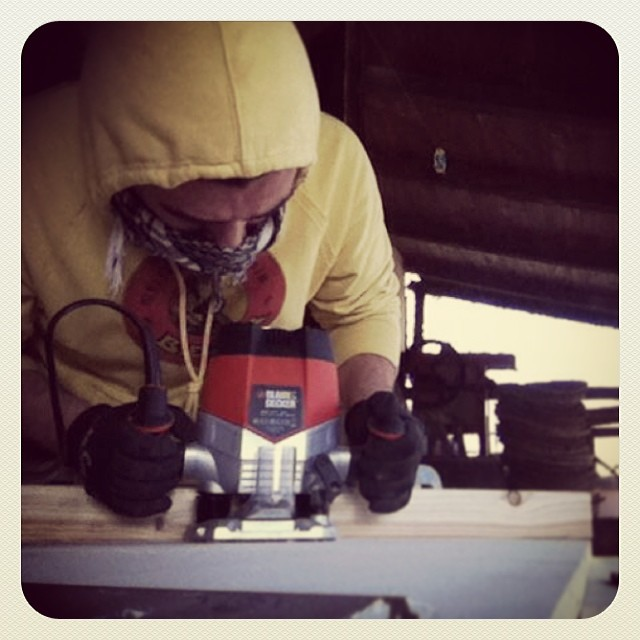
\includegraphics[width=.50\textwidth]{img/image2.jpg}
		\caption{Mappa della disposizione dei microfoni realizzata da Gabriele Acquafredda}
		\label{gs}
	\end{figure}
	
	\subsection{Ruoli di ciascun punto di ripresa}
	Ciascuno dei microfoni ha un ruolo preciso all'interno della ripresa dell'orchestra, in base a due parametri principali, ovvero:
	\begin{compactitem}
		\item Coppia stereofonica della quale è parte
		\item Il suo \textbf{posizionamento} nello spazio: essendo i microfoni utilizzati identici tra loro (fatta eccezione per l'ORTF), il loro carattere dipende solo ed esclusivamente dal loro posizionamento.
	\end{compactitem}
	È solo in base a questo che la sonorità dell'ambiente e della fonte sonora cambia nella ripresa.
	
	\subsubsection{L'ORTF}
	Il punto di ripresa principale è costituito da un ORTF, ovvero una coppia stereofonica semi-spaziata formata da due cardioidi posti ad una distanza di 17cm tra di loro (circa la stessa distanza che intercorre tra le orecchie in un cranio umano) inclinate di 110° circa.
	La caratteristica principale della configurazione ORTF è la sua \textbf{naturalezza}: dato il ritardo tra le due capsule microfoniche, questa coppia semi-spaziata permette di riprendere una fonte sonora in maniera tridimensionale, fornendo informazioni relative alla profondità dell'ambiente acustico nel quale suona.
	In questo caso, L'ORTF è stato posto di fronte all'orchestra in corrispondenza del pianoforte e del direttore, a fronte palco.
	
	\subsubsection{I 10 Line Audio modello OM1}
	Osservando il diagramma polare e la risposta in frequenza del microfono omnidirezionale di marca Line Audio modello OM1 mostrato nella figura 2, si può evincere che questo microfono \textbf{non è lineare in direzionalità}: si comporta diversamente a seconda delle frequenze che riprende, stringendo la sua figura polare. Dal diagramma si può notare che il microfono è realmente omnidirezionale a 125 e a 2000 Hz, la sua figura polare si stringe di poco a 250 e a 4000 Hz. A 500 e a 8000, in particolar modo sul retro, la figura si stringe ancora sino ad essere attenuata di quasi 10dB a 1KHz e a 16KHz.
	
	\begin{figure}[h]
		\begin{center}
			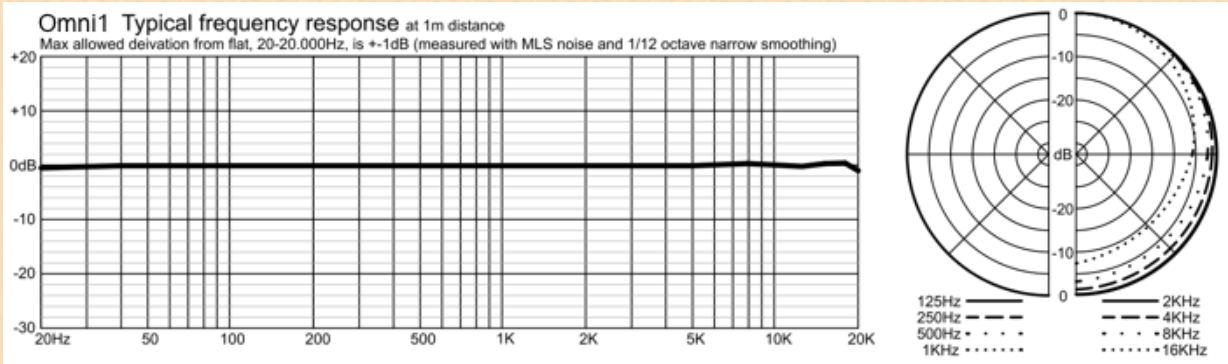
\includegraphics[width=.47\textwidth]{img/image1.png}
			\caption{\textbf{Caratteristiche del microfono di marca Line Audio modello Omni1}. Diagramma polare e risposta in frequenza.}
			\label{gr01}
		\end{center}
	\end{figure}
	
	Nonostante questa caratteristica, la scelta di utilizzare dei microfoni omnidirezionali è funzionale a fornire una ripresa \textbf{tridimensionale} dell'orchestra, in quanto saranno riprese anche le riflessioni dell'ambiente acustico circostante con le sue caratteristiche riverberanti. Ciò significa che saranno fornite informazioni relative a come la fonte sonora ripresa interagisce con l'auditorium anche alle spalle del microfono, essendo quest'ultimo, appunto, omni-direzionale.
	
	I 10 microfoni sono stati organizzati in coppie stereofoniche AB, la quale prevede che essi siano distanziati ad una distanza variabile in base alle dimensioni della sorgente. In particolar modo:
	
	\begin{enumerate}
		\item Una coppia per i primi violini e per le viole, posizionati specularmente nell'orchestra a distanza di 425cm l'uno dall'altro.
		
		\item Per la sezione dei fiati sono stati utilizzati tre microfoni, dei quali uno centrale e due laterali, per due motivi principali:
		\begin{compactitem}
			\item La sezione è molto ampia(428cm), dunque per evitare di avere un buco nella ripresa del centro della sezione, è stato aggiunto un microfono al centro del fronte.
			\item Per catturare anche i timpani, e in particolar modo il loro dettaglio timbrico, essendo storicamente utilizzati per dare sostegno ai fiati aggiungendo attacco e corpo al  suono.
		\end{compactitem}
		
		\item Una coppia a distanzata di 28cm per il pianoforte. Questa coppia è molto stretta rispetto alle altre perchè ha come intento quello di riprendere il pianoforte come oggetto centrale nell'immagine.
		
		\item Due utilizzati come Flanks, a distanza speculare di 324cm per allargare l'immagine stereo dell'ORTF. Il complesso Flanks + ORTF costituisce la ripresa MAIN dell'orchestra, ovvero quella generale, la quale serve a dare un'immagine complessiva frontale del corpo dell'orchestra e a riprendere l'interazione di quest'ultima con l'auditorium.
		
		\item Uno come spot per i contrabbassi, posto a 309cm dal flankR. La sua utilità sta nell'aggiungere il loro dettaglio alla ripresa complessiva. C'è da precisare che questo punto di ripresa non potrebbe dare informazioni sulla profondità della sezione trattandosi di un microfono mono, così come non potrebbe riprenderne fedelmente le basse frequenze essendo un microfono di spot e quindi molto vicino alla sorgente.
	\end{enumerate}
	
	\section*{Valutazione della ripresa}
	Ora che conosciamo le distanze tra i microfoni, le tecniche e i microfoni utilizzati, le mappature di questi ultimi sul palco, e la posizione delle sezioni dell'orchestra nello spazio, possiamo fare una valutazione complessiva della ripresa in base a tre parametri:
	
	\subsection*{Direzionalità}[I]
	Ovvero capacità della ripresa di rappresentare fedelmente la \textbf{larghezza} di una fonte sonora e la \textbf{provenienza} longitudinale dei suoni. Nel nostro caso, l'intento è quello di riprendere delle sezioni di dimensioni medio-grandi, di conseguenza abbiamo bisogno di utilizzare delle coppie stereofoniche che siano spaziate a dovere. Attenzione però: il pericolo di distanziare troppo due microfoni tra di loro comporta due rischi:
	\begin{compactitem}
		\item Rappresentare l'immagine più larga di quanto in realtà non sia
		\item Creare un buco nella ripresa del centro
	\end{compactitem}
	Per evitare questi problemi, sono state adoperate delle soluzioni:
	\begin{compactitem} 
		\item La ripresa di una sezione larga come quella dei fiati è stata rafforzata con un microfono centrale.
		\item La ripresa principale dell'ORTF è stata allargata con dei Flanks
		\item La ripresa del pianoforte è molto più stretta rispetto alle altre
	\end{compactitem}
	
	\subsection*{Profondità}[II]
	Ovvero la capacità della  ripresa di rappresentare fedelmente la posizione delle sezioni dell'orchestra lungo la terza dimensione: quella della profondità.
	Nel nostro caso, questa percezione è data dalla relazione tra il fronte della ripresa e i lati della stessa: le informazioni stereofoniche ci sono fornite dalla relazione tra suono principale e suono riflesso.
	
	\subsection*{Ambiente}[III]
	Ovvero il corretto bilanciamento tra la definizione timbrica delle sezioni e la loro interazione con l'auditorium. Questo dipende principalmente da due fattori:
	\begin{compactitem}
		\item L'acustica dello spazio
		\item La distanza dei microfoni dalla sorgente
	\end{compactitem}
	Nel nostro caso, entrambe le condizioni sono favorevoli ad un buon bilanciamento del riverbero, in quanto:
	\begin{compactitem}
		\item L'acustica dell'auditorium è estremamente curata(nella forma, nelle sedute, nell'assorbimento e nella diffusione)
		\item La contemporanea ripresa della sorgente con microfoni ravvicinati(punti di ripresa delle singole sezioni) e microfoni lontani (punto di ripresa MAIN) permette un buon bilanciamento
	\end{compactitem}
	
	\section*{Scelta del dominio}
	Ora che abbiamo constatato come le tecniche di ripresa utilizzate rispecchiano il concetto di solidità desiderato al fine di ottenere una rappresentazione stereofonica del complesso orchestra/auditorium, analizziamo i due domini presi in esame per comprendere quali possibilità aprono per indagare l'immagine stereofonica.
	
	\subsection*{Dominio Sinistra/Destra}
	Ascoltare la ripresa nel dominio Sinistra/Destra vuol dire disporre longitudinalmente le riprese nell'immagine di ascolto senza sfruttare al meglio le informazioni stereofoniche al fine di costruire un'immagine abbastanza larga dell'orchestra.
	É chiaro che le possibilità di analisi e di gestione del materiale al fine di rappresentare le riprese quanto più fedelmente possibile all'immagine reale dell'orchestra sono di conseguenza limitate.
	Questa configurazione permette di processare i segnali con diversi approcci all'equalizzazione o alla compressione ad esempio, ma la possibilità di gestione dell'immagine stereofonica non è ricca come nel caso del dominio Mid/Side.
	Nella figura 3 è riportato il grafico dell'andamento della larghezza dell'immagine stereofonica durante una precisa sezione(A) delle riprese effettuate, nonchè la medesima utilizzata per svolgere la stessa indagine nel dominio Mid/Side, riportato invece in figura 4.
	
	\begin{figure}[h]
		\begin{center}
			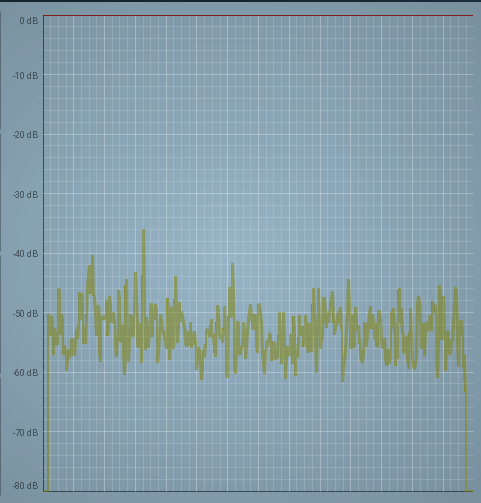
\includegraphics[width=.47\textwidth]{img/image3.png}
			\caption{\textbf{Grafico dell'andamento della larghezza dell'immagine stereofonica in configurazione Sinistra/Destra}. Sezione A della ripresa.}
			\label{gr01}
		\end{center}
	\end{figure}
	
	\subsection*{Dominio Mid/Side}
	Perchè analizzare il materiale delle registrazioni in Mid/Side?
	In questa configurazione, si può indagare l'ambiente come uno spazio trigonometrico, in quanto è possibile percepire la profondità dell'orchestra nell'auditorium nel quale suona grazie alla relazione tra centro ed estremi delle riprese, rimanendo fedeli al concetto di stereofonia.
	A differenza del dominio Sinistra/Destra, questa rappresentazione delle riprese costruisce un'immagine d'ascolto più fedele a quella reale in termini di ampiezza, e questo apre diverse possibilità relative alla gestione dell'immagine stereofonica.
	
	\begin{figure}[h]
		\begin{center}
			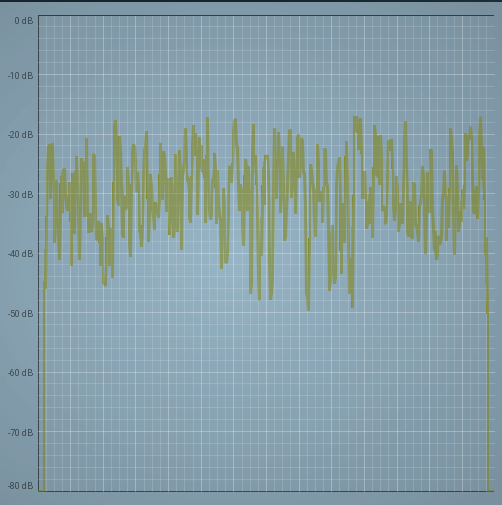
\includegraphics[width=.47\textwidth]{img/image4.png}
			\caption{\textbf{Grafico dell'andamento della larghezza dell'immagine stereofonica in configurazione Mid/Side}. Sezione A della ripresa.}
			\label{gr01}
		\end{center}
	\end{figure}
	
	In fase d'ascolto, è utile mettere in correlazione le diverse coppie stereo con il punto di ripresa MAIN per potersi fare un'idea del posizionamento che  queste assumono nella profondità dell'immagine stereofonica.
	Di seguito alcuni esempi:
	\begin{compactitem} 
		\item [I FIATI] Mettendo in solo il complesso MAIN, si può notare come l'immagine acquisisca profondità quando viene acceso il gruppo dei fiati. Si ha come l'impressione che un velo teso di suono venga allungato in profondità. Si rafforza il Mid e si percepisce meglio il dettaglio timbrico dei fiati e dei timpani.
		\item [VIOLINI E VIOLE] In questo caso, attivando il gruppo AB di Violini e Viole e sovrapponendolo al complesso MAIN, il complesso acquisisce profondità e si percepisce la totalità dell'orchestra. In questo caso il Mid è più debole rispetto ai fiati.
	\end{compactitem}
	Il Mid/Side è una rappresentazione grazie alla quale è possibile percepire al contempo tutte le informazioni stereofoniche riprese in fase di registrazione: direzionalità, profondità, ambiente, corpo e dettagli timbrici.
	
	\subsection*{Indagini Mid/Side}
	Indagare il materiale in Mid/Side equivale a poter dominare una maggior quantità di possibilità nell'elaborazione del segnale.
	Raggruppiamo le tracce in diverse folder tracks e vediamo degli esempi:
	\begin{compactitem} 
		\item MAIN(ORTF, Flanks)
		\item FIATI(Fiati Left, Fiati Right, Fiati Center)
		\item VIOLINI/VIOLE(Secondi Violini, Viole).
		\item PIANOFORTE (Piano Left, Piano Right)
	\end{compactitem}
	Gestire separatamente Mid e Side, dà la possibilità di intervenire sull'ampiezza dell'immagine stereofonica con maggior efficacia:
	\begin{compactitem}
		\item Si può comprimere il Mid per rafforzare il centro della ripresa laddove ce ne fosse bisogno, come ad esempio nel caso del complesso Violini/Viole.
		\item Si può aggiungere un leggero riverbero al Mid per poter invece allargare  l'immagine
	\end{compactitem}
	
	Questo dominio apre anche diverse possibilità relative all'equalizzazione.
	Con il fine di far emergere il dettaglio delle diverse sezioni dal timbro delle regitrazioni, le si può filtrare in maniera non invasiva: nelle riprese Mid dei \textbf{fiati} è possibile attenuare le frequenze gravi, in quanto l'utilità di questo punto di ripresa sta anche nel riprendere il dettaglio timbrico dei fiati e delle membrane dei timpani, i quali servono a sostenere i fiati. Le frequenze gravi dei timpani saranno già riprese fedelmente dai microfoni MAIN, trattandosi di microfoni lontani, dove la loro distanza dalla sorgente sonora permette a quest'ultima di svilupparsi per tutta la sua lunghezza d'onda.
	
	\section*{Conclusioni}
	In conclusione, il requisito fondamentale per ottenere una buona resa stereofonica nella rappresentazione delle riprese, è la qualita di queste. Non si possono costruire reali informazioni stereofoniche relative all'ambiente nella sua ampiezza o profondità senza riprenderle adeguatamente.
	Tuttavia, vengono aperte diverse possibilità di analisi in base al dominio scelto per la rappresentazione.
	
	
	\vfill\null
	
	\newpage % USE NEWPAGE TO FORCE COLUMNN INTERRUPTION
	%-------------------------------------------------------------------------------
	%-------------------------------------------------------------------------------
	
	%--------------------------------------------
	%----------------larghezza massima del codice
	
	\vfill\null
	
	\raggedright
	%\bibliographystyle{unsrt}
	%\printbibliography
	
\end{document}

%%%%%%%%%%%%%%%%%%%%%%%%%%%%%%%%%%%%%%%%%%%%%%%%%%%%%%%%%%%%%%%%%%%%%%%%%%%%%%%%
% 2020 GIUSEPPE SILVI ARTICLE TEMPLATE BASED ON
%%%%%%%%%%%%%%%%%%%%%%%%%%%%%%%%%%%%%%%%%%%%%%%%%%%%%%%%%%%%%%%%%%%%%%%%%%%%%%%%
% Journal Article
% LaTeX Template
% Version 1.4 (15/5/16)
% This template has been downloaded from:
% http://www.LaTeXTemplates.com
% Original author:
% Frits Wenneker (http://www.howtotex.com) with extensive modifications by
% Vel (vel@LaTeXTemplates.com)
% License:
% CC BY-NC-SA 3.0 (http://creativecommons.org/licenses/by-nc-sa/3.0/)
%%%%%%%%%%%%%%%%%%%%%%%%%%%%%%%%%%%%%%%%%%%%%%%%%%%%%%%%%%%%%%%%%%%%%%%%%%%%%%%%
